\chapter{可解释性}
\label{chap:trust-interpretability}

一封邮件被模型拦截后，不同的人会拿“解释”去回答完全不同的问题，而没有一种解释能同时满足所有问题。用户想知道“这封邮件到底是哪些内容触发了拦截”，这是针对单次决定的解释；开发者怀疑模型在一整类邮件上依赖了不稳定的页脚，想确认这个规律是否普遍存在，这是针对整体行为的解释；受影响的发件人则只想知道“我现在能做什么把邮件恢复”，这需要可执行的补救方案。三者之间有联系——开发者也可以从某一次误拦出发提出假设，再到指定范围的邮件上用依赖指标检验——但它们需要的证据不同，一张特征热力图不能自动覆盖这三种用途。

按第~\ref{chap:trust-foundations}章的三层架构，可解释性主要提供支持理解、质疑与补救的证据。属性或规范层先确定要解释哪个行为、解释给谁、用来支持什么决定；生命周期层还要检查解释可以向谁公开、模型版本变化后是否仍然成立、以及在有人有意规避时能否保持。因此解释本身也是有使用条件的产物，不是“给出一张图”就结束。

\term{可解释性}（interpretability）研究的是人能否借助适当的表示和证据理解模型行为。它与前几章的关系要摆正：第~\ref{chap:trust-robustness}章用模板变化暴露捷径、上一章评价并约束行为，本章进一步定位这些行为究竟依据什么；但一次模型失效只能提出“为什么”的问题，答案还需要相应方法核验，不能凭直觉补一个故事。本章先区分解释的目的与范围（15.1），再分别介绍整体解释（15.2）、单次解释（15.3）、解释质量的检验（15.4）和行动补救（15.5）。第~\ref{chap:trust-reliability}章的预测可靠性提供相关但不同的证据：解释合理不代表预测可靠，反之亦然。

\section{模型的可解释性}
\label{sec:interpretability-purpose}

\subsection{解释对象决定证据}

提出任何解释之前，先要回答三个前置问题：解释什么（哪一项输出或哪条规律）、交给谁（开发者、普通用户还是寻求补救的人）、支持什么判断（调试、质疑还是采取行动）。不同接收者需要的粒度差别很大：开发者可能要看内部激活和相关训练样本，普通使用者可能只需要“哪些因素相关、适用范围是什么”，寻求补救的人则需要“我能改变什么”。信息粒度要与任务匹配，解释的价值不取决于列出的因素多少。

这里必须把三个层次分开，它们最容易被一句“某特征影响了结果”混为一谈。其一是模型行为：年龄与输出相关，这只是对观测到的输入—输出关系的描述。其二是模型内部的计算机制：在模型输入中人为修改年龄字段，可以检验模型这个系统怎样使用该字段。其三是现实因果：现实中改变一个人的年龄通常不可行、也不该作为建议行动，更不能从字段上的扰动试验推出真实世界中年龄导致了什么后果。使用“影响”一词时，应说清比较对象是什么、干预发生在模型内部还是现实世界。

\subsection{整体解释与单次解释}
\label{sec:interpretability-global-local}

\term{整体解释}（global explanation）用可理解的形式概括模型在某个明确的输入集合或参考分布上的判断规律，例如一组可执行规则、一条特征响应曲线，或某个概念的作用统计。“整体”指的是声明的覆盖范围——可以是全部部署邮件，也可以只是某种语言或某类业务邮件，并不意味着覆盖整个宇宙。它不要求逐项复述内部计算，但也不能因为是平均摘要就把结论推广到集合内的每一个输入。

\term{单次解释}（local explanation，常译“局部解释”）则固定一项具体输出，例如当前这封邮件为什么被拦截。常用办法是比较输入邻域、计算相对某个基准的分数差、或分析某次运行中各部分的计算作用；几何邻域只是构造参照的一种选择，不是必须。两类解释都需要可核查证据：整体主张要交代总体覆盖范围和抽样，单次主张要固定参照、邻域或具体的一次运行条件。

整体和单次之间可以互相转化，但方向要分清。一条准确的整体加性规则可以直接代入当前特征解释这一次预测；多次单次归因在定义固定后也可以汇总成整体摘要。但反方向不成立：作用方向相反的子群可能在平均中互相抵消，单个案例无论多典型都不能支持普遍规律。还要注意“解释范围（整体/单次）”和“能访问什么（只查输入输出/能看参数）”是两个独立维度，输入输出查询既可以做整体也可以做单次解释。

\begin{example}[同一规则的整体与单次说明]
\label{ex:interpretability-global-local}
示例~\ref{ex:interpretability-global-local}用一个极简评分器把两种解释放在一起。设二元特征$x_1$表示邮件是否有支付要求、$x_2$是否带可执行附件，评分规则为$f(x_1,x_2)=1+2x_1+4x_2$，分数达到6就隔离（这里分数只是内部评分，不是概率）。整体解释给出基准分1、两项各自的增量2和4、以及阈值6，覆盖四种输入组合；对当前邮件$(1,1)$的单次解释则是直接代入$1+2+4=7$，相对基准$(0,0)$两项贡献分别为2和4。代入只解释了这一次计算；要断言它就是真实模型的整体规则，还需要模型结构或大量查询证据支持。
\end{example}

图~\ref{fig:trust-global-local-explanation}把这两件事画开：左侧列出四种输入组合下的规则，右侧只对当前$(1,1)$代入计算，两者承担的核验任务不同。

\begin{figure*}[htbp]
  \centering
  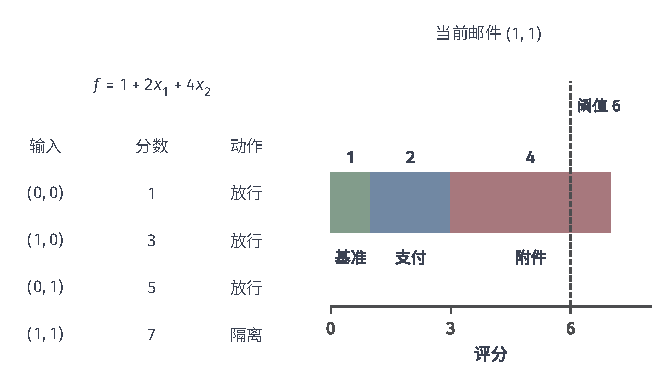
\includegraphics[width=113.404mm]{figures/03-foundations/03-trustworthiness/tikz/trust-global-local-explanation/figure.pdf}
  \caption{示例~\ref{ex:interpretability-global-local}的规则覆盖与代入。左侧列出四种组合的规则，右侧对$(1,1)$计算基准1加贡献2、4，得到7并与阈值6比较。计算分数不作概率解释，特征贡献也未表达现实因果作用；单次代入与整体覆盖分别需要核验。}
  \label{fig:trust-global-local-explanation}
\end{figure*}

\subsection{解释的表示与证据条件}

“结构简单”并不自动等于可理解，还要看操作的特征有没有明确含义。一个稀疏线性式或一张短规则表，如果操作的是上万个没有名字的嵌入维度，使用者仍然无法理解。反过来，一个复杂模型在局部也可能被简单规则相当准确地近似，但这个近似的有效范围必须限定在已验证的区域，不能外推。

能访问什么信息，决定了能给出什么强度的证据：只有输入输出查询，只能做行为层面的近似；能访问参数和激活，才可能提出关于计算机制的假设；能重新训练模型，则可以更直接地检验数据的影响。读后面的方法时，应先核对它需要什么访问条件，再判断它能回答哪一类问题——不要拿行为近似的结果去声称机制。

解释还隐含一个常被忽略的要素：参照系。“这封邮件为什么被拦而那封相似邮件没有”是在两封邮件之间作输入比较；“为什么隔离而不是转人工复核”则是在两个行动之间作比较。两类问题需要不同的背景、分数和约束，即使同一个归因算法，换一个基准也会给出不同答案。交付解释时应列明：解释的是哪个输出、给谁、支持什么判断或行动、参照是什么、输入范围多大、哪些因素允许变化。

\section{整体行为的解释}
\label{sec:interpretability-global}

整体解释可以围绕三个不同的对象展开，它们回答的问题依次深入：模型的计算结构是怎样把输入组合成输出的（15.2.1，基于结构）；可观察的输入因素变化时输出如何响应、破坏某因素会带来多大性能损失（15.2.2，基于输入）；这些输入因素背后对应什么人能理解的语义概念（15.2.3，基于语义）。三方面可以结合（例如一个可读结构直接在命名概念上计算），所以下面的分类依据是“主要解释对象”，不是把模型分成互斥的类型。

\subsection{基于模型结构的解释}
\label{sec:interpretability-global-response}

想解释整套计算规则，有两条根本不同的途径。一是直接使用一个本身可读的预测器（加性模型、小树、规则表），这时要验证它的任务表现是否够用、人是否真能读懂其结构；二是保留复杂的原模型、在训练后另拟合一个可读代理去模仿它，这时除了可理解性，还必须检验代理与原模型到底有多相符。解释中必须写明规则到底来自哪个模型，否则读者会误以为代理规则就是原模型的真实计算。

\term{广义加性模型}（generalized additive model, GAM）是第一条途径的代表，它把预测分解成若干单特征函数之和，使每个特征的作用可以单独画成一条曲线查看：
\begin{equation}
 f(\bm{x})=\beta_0+\sum_{j=1}^{d}f_j(x_j)\, .
 \label{eq:interpretability-gam}
\end{equation}
其中$\beta_0$是基准分，$f_j$是第$j$个特征的响应函数。回归时$f$直接作为预测值，二分类时把它当作对数几率再经逻辑函数转成概率。为使各$f_j$的大小可以比较，要固定中心化约定（例如让每条曲线在训练分布上均值为零）。曲线斜率表示模型在该处对该特征的敏感性，而把样本覆盖情况画在曲线上，可以区分哪些形状有数据支撑、哪些区域只是估计不稳的外推\scite{hastie1986gam}。

纯相加结构的限制发生在式~\eqref{eq:interpretability-gam}的分数尺度上：某个特征带来的分数增量不能随另一个特征改变。仅仅“两个因素单独出现都正常、同时出现被隔离”，还不能证明存在这种交互；前面的加性教学规则经过阈值6之后就有这一现象。要看清限制，可以另设一个二值分数例：$f(0,0)=f(1,0)=f(0,1)=0$而$f(1,1)=1$。若它能写成常数与两个单变量函数之和，就必须有$f(1,1)-f(1,0)-f(0,1)+f(0,0)=0$，但这里该差为1，因此不能如此分解。分类概率还经过逻辑函数变换，讨论加性与交互时应先说明是在分数、对数几率还是概率尺度上。Lou 等在单变量项之外加入少量二元函数$f_{j,k}(x_j,x_k)$，用二维曲面表示交互。训练时要选择加入哪些交互并控制复杂度，解释时也应同时展示单项曲线和交互曲面，不能只报其一\scite{lou2013ga2m}。

决策树和规则表同样可以让人追踪决策路径，但规则数量、重复条件和深度会迅速增加阅读负担；只展示几条常见路径又会遗漏低频但可能关键的分支。因此是否采用可读结构，应在具体任务中同时比较它的预测损失和使用者依据它判断的实际表现，模型复杂度数字本身不能替代这种比较。

这里要澄清一个训练视角的常见疑问。训练实际预测器时，真实标签只作为监督信号进入损失或拟合过程；部署后预测器读取的只有输入特征，并不会读取待预测样本的真实标签。可以在加性、平滑性、树深度等结构限制下训练预测器，训练完成后解释展示的就是它的函数、阈值和交互如何组合出输出。可理解性来自“这些规则和特征能够被追踪”，不能仅因训练方法名字里带“可解释”就认定它易懂。

第二条途径是为复杂模型在声明的分布上建立一个\term{整体代理}（global surrogate）。做法是从该范围抽取输入，查询原模型$f$得到分数，再用这些分数（而不是真实标签）在可读模型族$G$（浅树、规则、加性模型）中拟合一个$g$。令$\Omega$惩罚复杂度、$\lambda\geq0$控制拟合与简洁的权衡，一种目标为
\begin{equation}
 \hat g=\argmin_{g\in G}\left\{
 \frac1n\sum_{i=1}^n\bigl[f(\bm{x}_i)-g(\bm{x}_i)\bigr]^2
 +\lambda\Omega(g)\right\}\, .
 \label{eq:interpretability-global-surrogate}
\end{equation}
注意拟合目标是原模型的输出$f(\bm x_i)$，不是真实标签$y_i$：用$y_i$另训一个小模型得到的是一个独立的新模型，并不构成对$f$的解释。分类问题中代理可以拟合概率也可以拟合类别，选择不同保留的东西不同——拟合概率保留分数变化，拟合类别只保留决策边界。

代理要交付它实际学到的规则，并在另外留出的查询样本上比较$g$与$f$的差异。示例~\ref{ex:interpretability-global-local}的真实规则可以由一棵“先看附件、再看支付要求”的树准确复述；但一棵简化成“有附件就隔离”的树会在$(0,1)$（无支付要求、有附件，真实分5不隔离）上出错。即使整体平均一致率达到预设阈值，也必须检查关键业务分支是否被近似错；可以提高代理复杂度或收窄声明范围来改善，但要同时报告因此增加的理解负担。

\subsection{基于输入的解释}
\label{sec:interpretability-global-dependence}

代理模型给出的是可以重新计算的近似规则；另一类整体解释不追求复述规则，只回答“某个因素起什么作用”这一特定问题。这里又有两种问法：一是把特征取值人为改变、看分数如何响应（描述函数形状，不需要真实标签）；二是破坏掉某条信息、看任务损失变化多少（描述模型性能对该信息的依赖，需要真实标签）。两者所需标签和判断尺度不同，不能互相替代。

\paragraph{响应形状与交互}

\term{部分依赖}（partial dependence, PD）回答第一种问法：把目标特征固定在某个取值，对其他特征按参考分布取平均\scite{friedman2001gradientboost}。设输入参考分布为$P_{\mathrm{ref}}$、$\bm X\sim P_{\mathrm{ref}}$，对其支持范围内的$t$定义
\[
 \operatorname{PD}_j(t)
 =\mathbb E_{\bm X_{-j}\sim P_{\mathrm{ref},-j}}
 f(t,\bm X_{-j})\, .
\]
其中$\bm X_{-j}$是其他特征，$P_{\mathrm{ref},-j}$是其边缘分布。这个定义同时固定了两件事——被替换的是哪个字段、对哪个人群平均，曲线必须连同这两个条件一起解读。

经验上，从参考总体采样，在每个$t$处把所有样本的第$j$个字段替换成$t$再查询模型并平均：
\[
 \widehat{\operatorname{PD}}_j(t)
 =\frac1n\sum_{i=1}^n f(t,\bm{x}_{i,-j})\, .
\]
把均值按$t$连起来，可以看出阈值、单调性或饱和等形状；对两个特征在二维网格上重复操作可以检查交互。除了平均曲线，还应查看个体条件曲线，因为不同子群的响应方向可能相反，平均会把它们抵消掉。

用教学规则算一遍：四种组合等概率时，$\operatorname{PD}_1(t)=3+2t$、$\operatorname{PD}_2(t)=2+4t$（例如固定$x_1=t$后对$x_2$平均，基准和$x_2$的期望贡献合并成截距3）。它给的是平均分数响应，既不预测每封具体邮件，也没有用真实标签检验模型是否正确。换参考人群会改变截距；这个例子没有交互，所以两条曲线斜率仍分别是2和4。

PD有一个根本隐患：人为替换可能造出数据中根本不存在的输入。例如数据里恒有$x_1=x_2$，模型$f(x_1,x_2)=x_1-x_2$在真实观测上总输出0；单独把$x_1$改掉，PD曲线却会上升。这条曲线描述的是模型在人工组合上的响应，不能当作观测人群中的现实效应。

一种修正是把其他特征按目标特征的取值做条件化（只在$x_j$附近的真实样本上平均），减少人工无效组合，但这样会把特征之间的关联纳入平均，回答的问题随之改变。因此应明确用的是边缘分布还是条件分布；即使两条曲线形状相似，也不能据此断定它们解释的是同一种作用。

\term{累积局部效应}（accumulated local effects, ALE）用另一种思路减少外推：不把特征整个替换成任意$t$，而是在每个样本现有取值附近估计“小幅变化引起的输出变化”，再沿特征轴把这些局部变化累积起来\scite{apley2020ale}。为严格表述，限定连续特征的一个有界区间$I$，把参考总体限制为$P_{\mathrm{ref}}(X_j\in I)=1$，并设$X_j$的密度在$I$上几乎处处为正；假设模型对第$j$维可微，并可选择关于$s$可测的条件导数均值。为使后面的累积与中心化都有定义，再明确要求
\[
 \int_I\mathbb E_{P_{\mathrm{ref}}}\!\left[
 \left|\frac{\partial f(s,\bm X_{-j})}{\partial s}\right|
 \,\middle|\,X_j=s\right]\mathrm ds<\infty.
\]
这里先在给定$X_j=s$的分布中对其他特征取期望，再按特征轴上的长度积分；不是只要求每个$s$处的条件期望分别有限。这个条件使所有子区间的累积量有统一有限上界，因而随后对$X_j$取中心化期望也有限。对$t_0,t\in I$，其一阶形式为
\begin{equation}
 \operatorname{ALE}_j(t)
 =\int_{t_0}^{t}
 \mathbb E_{P_{\mathrm{ref}}}\!\left[
 \frac{\partial f(s,\bm X_{-j})}{\partial s}
 \,\middle|\,X_j=s\right]\mathrm ds-C_j\, ,
 \label{eq:interpretability-ale}
\end{equation}
其中$t_0$是积分起点，$C_j$是中心化常数，使整条曲线在同一参考分布下均值归零。正密度条件保证条件均值的不同版本只在零测集上有差别、不影响积分；绝对可积保证累积值和中心化常数有限（相关条件可参考\BookChapterRef{chap:random-variables}{卷2《数学准备：概率、因果与决策》第1章“随机变量”}）。实际计算不必求导：把取值分箱，在每箱内用已有样本查询“箱上边界减箱下边界”的输出差，累加这些平均差即可。离散特征或没有数据的区间要另行声明差分或外推约定，不能从这个积分式自动得到。

一句话对比：PD平均的是完整输出（需要人造输入），ALE平均的是局部变化（尽量贴着数据走）。ALE减少了外推，但也有自己的问题：分箱太粗可能一步跨过无数据区，太细又可能每箱样本不足；模型在数据流形之外的延伸仍可能影响局部导数。和PD一样，ALE识别的也不是现实因果作用。保留个体响应曲线有助于检查总体均值遗漏的交互。

\paragraph{任务表现对信息的依赖}

上面的曲线都没用真实结果，所以它们说明不了“模型对这个特征敏感是否有助于正确分类”——模型完全可能强烈依赖一个无用特征。要检验模型是不是靠页脚才判断正确，必须固定同一个模型，比较保留页脚和破坏页脚两种情况下的任务损失，这个问题以任务表现为依据，系数大小回答不了。

\term{置换重要性}（permutation importance）就是这种性能依赖检验：固定模型不动，把测试样本中某个字段的取值随机打乱（破坏该字段信息但不改模型），比较打乱前后的任务损失\scite{breiman2001randomforests,strobl2007bias}。应在同一批样本上成对计算、重复多次置换，报告损失增量及其波动。损失增量超过预设阈值，支持的是“在这种破坏规则下模型性能依赖该字段”；这种依赖是否合理、有没有现实因果意义，仍需另外判断。

设$\pi$是样本索引的一个排列，$\bm x_i^{(j,\pi)}$表示把第$i$个样本的第$j$个字段替换成第$\pi(i)$个样本的该字段、其他字段不变，一次置换的损失增量为
\begin{equation}
 \widehat I_j^{(\pi)}
 =\frac1n\sum_{i=1}^n\left[
 \ell\bigl(f(\bm{x}_i^{(j,\pi)}),y_i\bigr)
 -\ell\bigl(f(\bm{x}_i),y_i\bigr)\right]\, .
 \label{eq:interpretability-permutation}
\end{equation}
这里$y_i$只用于计算任务损失，模型自始至终不重新训练。教学例：100封测试邮件中误判数由10升到25，置换重要性就是$0.25-0.10=0.15$。重复置换的结果波动反映置换随机性；推广到新邮件总体还要计入测试样本本身的抽样不确定性。

置换时要警惕破坏字段间的真实关联。页脚往往与发送方配套出现，单独置换页脚会造出“这个发送方从不使用的页脚”这种现实中不存在的组合，损失增量里就混入了分布外效应，而不只是“丢失页脚信息”。想研究“控制发送方后，页脚还能额外提供多少预测信息”，可在同一发送方内部置换页脚。这保持发送方不变，破坏的是同一发送方条件下页脚与结果的联系，并没有删除发送方字段；想研究“发送方加页脚整组信息”的作用，则联合置换整组。对于可以互相替代的字段还要小心：模型没使用的那个字段置换重要性可能为零，但它仍含预测信息；“删除字段后重新训练”检验的是学习系统能否利用替代信息，是另一个问题，应单独报告。

最后强调响应分析和性能依赖可以给出不一致的结论。分数对某特征很敏感，但变化没有越过分类阈值时，零一损失增量可能接近零；破坏一个被模型错误使用的特征甚至可能让损失下降。曲线描述模型怎样响应，置换损失描述这种响应对所选指标的实际后果，至于这种依赖任务上能否接受，则要由任务语义判断。

\subsection{基于语义的解释}
\label{sec:interpretability-global-concepts}

输入字段往往不等于人真正关心的含义。“催促立即转账”这个概念有很多种文字表达，同一个词也可能出现在引用他人诈骗话术或警示语中，按字段或词项统计难以直接回答“模型是否在对‘催促转账’作反应”。语义解释改用人能理解、来源可核验的概念（如催促付款、可验证来源）来组织证据：可以把这些概念放进模型的实际预测通路，也可以在模型已有的内部表示中检验某个概念方向是否起作用。

第一种做法是\term{概念瓶颈模型}（concept bottleneck model）：模型先预测一组人定义的概念，再只允许通过这些概念决定最终结果。这样语义接口成为计算的必经之路，概念的取值可以被查看和人工修改；它与“模型给完判断后再附一段概念描述”有本质区别，后者的描述不参与计算\scite{koh2020conceptbottleneck}。

设概念向量为$\bm c\in\mathbb R^m$、概念预测器为$g$、最终决策函数为$h$，模型结构为$f(\bm x)=h(g(\bm x))$。有概念标签时训练方式有多种选择：可以先训$g$，再用真实概念训$h$；也可以用$g$预测出的概念训$h$；还可以把任务预测和概念预测合成联合目标。这些选择各有陷阱：若$h$训练时看到的是真实概念、部署时接收的却是$g$的预测，就会产生训练—部署失配（$h$没见过概念误差）；用预测概念训练或联合训练则让$h$在训练时就暴露于概念误差，但误差分布将来变化时仍需复查。不同训练方式还决定任务信号会不会反过来改变概念预测器。部署中人工确认邮件来源后，可以直接替换对应概念值再看输出如何变化。

即使有了瓶颈，要解释整套规则仍须说明$h$如何组合这些概念（加性项、阈值或决策路径）；如果$h$本身很复杂，瓶颈只提供了可核查的接口，并没有自动展开全部计算。要概括某个概念的整体作用，应在目标任务样本上系统检验，而不是展示一次成功纠正就下结论。

命名接口也可能名不副实：概念本身的误判会向下游传播，概念定义遗漏会降低任务能力，而连续的概念分数中还可能夹带名称之外的信息。如果模型存在绕过瓶颈的旁路，替换概念也控制不了所有依据。验收时要共同核查概念本身的质量、替换概念后的效果和最终任务损失。

第二种做法不改造模型，而在模型已有的内部表示中检验语义假设，这就是\term{概念激活向量检验}（testing with concept activation vectors, TCAV）。Kim 等用“概念样本”和“对照样本”在某一激活层训练一个线性分隔器，其法向量$\bm v_C$指向目标概念方向；再统计目标类别的分数沿这个方向的导数为正的样本比例\scite{kim2018tcav}。它把“模型是否使用某概念”转成一个可重复的表示敏感性检验，不需要重训瓶颈模型。

设激活为$\bm h(\bm x)$、后续类别分数为$s_k(\bm h)$，TCAV 统计的就是方向导数$\nabla_{\bm h}s_k(\bm h(\bm x))^\top\bm v_C$的符号：正号表示沿概念方向移动时该类分数上升。样本、对照集和层的选择都会影响结果，应重复拟合并报告不确定性。还要认清它的局限：线性可分方向可能捕捉到的是与概念共现的背景而非概念本身；正导数只是内部局部敏感性，既不是对概念做现实干预的概率效果，也不限制模型只能使用所命名的概念。

实施时数据要分成三部分：概念实例和对照用来学习方向，目标任务样本用来测量作用，再另留样本复核。固定模型和层后，记录激活、训练线性分类器、确定指向正类的朝向，再对各目标样本计算方向导数。令$\bm D_k$为从声明的目标任务参考分布中、按预先规则纳入类别$k$分析的有限样本（例如要求真实标签为$k$且该层激活与梯度可算）；分母$|\bm D_k|$计入所有符合纳入条件的样本，而不只是导数为正的样本。汇总量为
\[
 \widehat t_{C,k}
 =\frac1{|\bm D_k|}\sum_{\bm{x}\in\bm D_k}
 \mathbb I\!\left\{
 \nabla_{\bm h}s_k(\bm h(\bm{x}))^\top\bm v_C>0
 \right\}\, .
\]
读法上要防止一个典型误读：100个样本中80个正导数得到0.8，意思是“八成样本在该概念方向上有正的局部敏感性”，绝不是“该概念贡献了80\%的分数”。更换概念实例和随机对照后，如果目标方向的比例持续高于随机方向，并报告差值与不确定性，才加强概念假设的证据。

小结三类整体解释：结构解释回答规则如何组合，输入解释回答字段起什么作用，语义解释回答这些字段对应什么人能懂的概念。概念瓶颈把命名概念放进真实预测通路，TCAV 用方向导数检验已有表示是否对概念敏感；两者都把语义概念与模型行为连起来，但改变的对象和提供的证据不同。无论哪类整体结论，都要交代样本覆盖、汇总规则以及方向相反的子群。

\section{单次行为的解释}
\label{sec:interpretability-local}

单次行为的“为什么”可以向三个方向追溯。针对误拦邮件：是输入中的哪些内容触发了判断（输入方向）；处理这封邮件时内部哪些组件参与了计算（计算方向）；训练集中的哪些样本使模型形成了这种判断（训练方向）。三类方法的解释范围都固定在当前这一次行为，但它们改变的对象不同。

相似案例、反事实、局部代理和归因都固定训练好的模型、只分析它对输入的响应；内部解释通过干预当前运行检查组件作用；数据解释则改变学习经历（删样本、改权重）再看同一输入结果是否变化。下面按“论断的对象”组织方法，至于方法只靠输入查询还是需要参数访问，只决定它在什么条件下能拿到证据。

解释前还要固定被解释的输出到底是什么：是连续的垃圾邮件分数、是隔离这个动作，还是“隔离与转人工复核之间”的选择。阈值和权限规则也参与最终动作的形成，只解释分数可能漏掉它们为什么越界。下文以$f(\bm x)$表示目标标量分数、$\hat y(\bm x)$表示经决策规则得到的类别或动作；多类别问题还须先固定解释哪个类别。

\subsection{基于预测输入的解释}
\label{sec:interpretability-local-input}

输入类解释通过检索参照样本或人为构造输入变化，把当前结果与输入差异联系起来：结果相同的近邻提示“这类输入共同导致该判断”，结果不同的近邻提示决策边界在哪，系统地改变输入则可以拟合局部响应或给各部分分配贡献。这些方法的共同对象是固定模型的输入输出，但交付的证据形式不同。

输入分析既可以检索原有样本，也可以读取导数，不一定要真的改动当前这封邮件。还要注意最终类别相同并不意味着分数没大变——分数可能波动很大但没越过阈值；因此解释时应记录自己比较的到底是分数、类别还是动作。

\paragraph{相似案例的对照}
\phantomsection
\label{sec:interpretability-local-examples}

\term{基于案例的解释}（example-based explanation）展示与当前输入相似、且模型判断相同的参照样本。例如支付要求和可执行附件共同触发隔离时，可以展示历史上同样包含这两项因素、被隔离的邮件，标出共同片段，让读者直观看到本次结果所属的案例组。

检索前先要定义“相似”按什么算：词语重叠、业务字段匹配，还是内部表示距离；哪些差异可以忽略。展示近邻时应给出距离、共同点和区别。若有真实标签，应同时展示标签和模型预测，避免把“相似的历史误判”当成当前判断正确的依据。展示多个近邻或有代表性的原型，可以减少偶然挑中一个特例的影响。

案例对照的证据强度取决于模型的预测机制。如果模型本身就是近邻投票或原型分类，展示的案例就是实际参与计算的对象，权重可以重算核验；如果案例只是在模型给出判断之后才检索来的，它们只提供线索，不构成依据。若要声称“正是这些共同因素解释了当前判断”，还必须实际改变这些因素并核对输出是否变化。

Chen 等的原型部件网络（ProtoPNet）属于前一种情况：它把图像各局部与学习到的原型比较表示相似度，再加权得到类别分数，原型直接关联训练片段\scite{chen2019protopnet}。因此可以显示当前图像区域对应哪个典型部件、贡献多少分，案例比较确实处在实际计算路径上。

使用时要警惕“相似”的内容可能不是读者以为的对象：相似性可能来自背景或邮件模板，而非业务意图中的关键物体。应展示模型实际比较的区域和贡献权重，减少读者自行猜测；同时展示“相近但输出不同”的案例，有助于检查决策边界。

\paragraph{不同结果的反事实比较}
\phantomsection
\label{sec:interpretability-local-counterfactual}

反事实比较研究的是“哪些差异足以改变当前判断”。可以检索真实存在的、结果不同的近邻（观察性对照），也可以只改少量条件后重新查询模型（受控变化）；后者通过控制其他因素，更直接地检验所改因素的作用。

Wachter 等的\term{反事实解释}（counterfactual explanation）把它表述成一个优化问题：搜索既接近当前输入、又能让输出变成目标类别的候选；可以最小化距离与目标损失，也可以把输出要求写成硬约束\scite{wachter2018counterfactual}。它把“为什么是这个结果”转换成“改成什么样会得到另一个结果”。

设目标输出集合为$Y_{\mathrm{target}}$、输入间距离为$d$、有效输入集合为$\bm X_{\mathrm{valid}}$，求
\begin{equation}
 \min_{\bm{x}'\in\bm X_{\mathrm{valid}}}
 d(\bm{x}',\bm{x}),
 \qquad \hat y(\bm{x}')\in Y_{\mathrm{target}}\, .
 \label{eq:interpretability-counterfactual}
\end{equation}
搜索可以从真实近邻、离散枚举或梯度方法入手；找到的候选必须通过完整预测流程重新核验，并明确列出改动了哪些字段。尺度、离散取值和哪些组合有效要预先确定，否则“最近”可能只是距离单位选择的产物（把年收入单位从元换成万元，最近点就变了）。有限搜索找到一个候选，既不证明它最小、也不证明唯一。

沿用教学规则：当前$(1,1)$得7分被隔离。把附件改成非可执行、保留支付要求得到$(1,0)=3$分；去掉支付要求、保留附件得到$(0,1)=5$分，两者都低于阈值6而放行。因此在其他项不变时，任一项改动都足以翻转结果；如果只展示“改附件”这一条方案，就会漏掉“改支付要求”这条同样有效的路径。

这些结论的适用条件要讲清：模型、参照和允许改动的范围都是固定的。多个字段同时不同的真实近邻只能提示差异，受控重算才能进一步检验预测作用。预测翻转也不等于现实因果后果或行动可行——“把字段改掉”在现实中未必做得到，行动条件要到第~\ref{sec:interpretability-recourse}节才补上。

为了单独看清“输入距离”这一层，图~\ref{fig:trust-counterfactual-nearest}改用后面补救章的连续申请例子：$s$为技能分数、$r$为当期资源，$s+r\geq3$时批准。当前$(1,1)$到批准区域的欧氏最近点是边界上的垂直投影$(1.5,1.5)$。这里只比较输入空间距离，完全没有计算达到该状态所需的培训成本和支持后果——那是补救问题。

\begin{figure}[!htb]
  \centering
  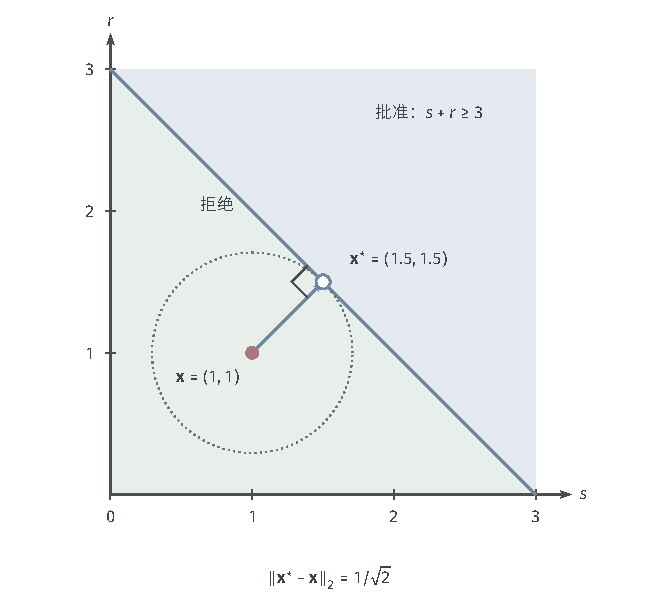
\includegraphics[width=\linewidth]{figures/03-foundations/03-trustworthiness/tikz/trust-counterfactual-nearest/figure.pdf}
  \caption{等权欧氏距离下的最近目标输入。从$(1,1)$到含边界$s+r=3$的批准区域，垂直投影为唯一最近点$(1.5,1.5)$，距离$1/\sqrt2$。虚线圆与直角记号分别显示等距和垂直关系。此处没有行动约束，实际补救路径另见图~\ref{fig:trust-actionable-recourse}。}
  \label{fig:trust-counterfactual-nearest}
\end{figure}

案例和反事实给的是具体参照；若要系统说明当前分数是怎么来的，还可以在输入邻域拟合一条简单响应规则（LIME），或把“当前分数相对某个基准的差”分配给各特征（IG、SHAP）。后面三类方法采用的都是某种比较，输出数值必须按各自定义的问题来解读。

\paragraph{附近输入的响应规则}
\phantomsection
\label{sec:interpretability-local-neighborhood}

\term{局部可解释模型无关解释}（local interpretable model-agnostic explanations, LIME）在当前输入附近查询模型、按样本与当前输入的接近程度加权，拟合一个简单的局部代理并惩罚其复杂度\scite{ribeiro2016lime}。它与整体代理的区别在于样本和权重：整体代理追求在整个分布上近似，LIME只追求在当前输入周围近似。

以邮件为例，用一个0/1词项保留向量$\bm z$表示“保留哪些词”，并通过$r(\bm z)$把向量还原成可查询的文本。设代理族为$G$、样本$\bm z_i$相对当前输入的接近权重为$w_{\bm x}$、复杂度惩罚为$\Omega$、$\lambda\geq0$，拟合目标为
\begin{equation}
 \hat g=\argmin_{g\in G}\left\{
 \sum_{i=1}^{n}w_{\bm x}(\bm{z}_i)
 \bigl[f(r(\bm{z}_i))-g(\bm{z}_i)\bigr]^2
 +\lambda\Omega(g)\right\}\, .
 \label{eq:interpretability-lime}
\end{equation}
这里有一个邻域宽度的取舍：把大权重集中在很窄的邻域，能更聚焦当前输入，但邻域内变化太少会导致各因素作用无法识别；放宽高权重邻域能看到更多变化，却可能超出简单模型能近似的范围。删词还可能破坏语法或改变任务本意，所以要核查邻域样本的有效性，并在另取的邻域样本上报告代理误差。拟合出的系数回答的只是“这个加权局部近似问题里各因素的系数是多少”。

LIME的计算流程是：先在可读的删词表示上采样一批变体，查询原模型对每个变体的分数，再按距离加权拟合出只有少量非零系数的代理。交付时应给出所选词项、系数和邻域近似误差；整个过程原模型参数保持不变。这些信息共同说明代理“在哪里、以多大误差”近似了当前响应。

在教学加性规则上，如果邻域样本足以分别识别两项作用，不加稀疏惩罚的线性拟合可以准确恢复系数2和4；但存在交互时，同一个词项的系数会随邮件内容变化，单一系数不再通用。与整体代理对照看：两者都是“查询后拟合”，整体代理的样本和误差覆盖整个分布，LIME的样本和误差集中在当前输入的权重邻域。

局部代理解释的是“附近输入怎样改变输出”；归因方法则换一个任务：标记当前输入中哪些证据在起作用，或把当前分数相对某个基准的差值分配给各特征。有些方法只标记敏感位置（不要求数值加和），有些则要求各项贡献之和等于规定的分数差；后一种要求依赖基准和“组合价值”的定义，数值必须据此解读。

\paragraph{扰动比较与局部敏感性}

遮挡（occlusion）用最直接的输入输出查询估计单项作用：按预先规定的参照替换第$j$项（文本替换片段、图像替换区域），比较替换前后的分数。交互作用和信息冗余会使“逐项移除的效果”加起来不等于总差值，因此替换规则本身必须写进解释定义。

对可微模型$f$，梯度描述当前点处小幅输入变化的瞬时敏感性。它有一个饱和问题：在激活饱和区域梯度可能接近零，但该特征可能在更早的阶段参与了分数形成；而且单点梯度不分配“相对基准的总差异”。要做分配，需要规定一条从基准到当前输入的路径，把沿途作用累积起来。

\paragraph{相对于基准的贡献分配}
\phantomsection
\label{sec:interpretability-local-attribution}

\term{积分梯度}（integrated gradients, IG）按这个思路设计：选一个基准输入$\bm x_0$（代表“没有信息”的状态），沿从基准到当前输入$\bm x$的直线路径积分每一维的梯度：
\begin{equation}
 \operatorname{IG}_j(\bm{x})
 =(x_j-x_{0,j})\int_0^1
 \frac{\partial f(\bm{x}_0+t(\bm{x}-\bm{x}_0))}
      {\partial x_j}\,\mathrm dt\, .
 \label{eq:interpretability-ig}
\end{equation}
令路径为$\bm\gamma(t)=\bm x_0+t(\bm x-\bm x_0)$、路径上的函数值为$\varphi(t)=f(\bm\gamma(t))$。如果$\varphi$在$[0,1]$上绝对连续，各坐标项可积，那么链式法则几乎处处给出
\[
 \varphi'(t)=
 \sum_j\frac{\partial f(\bm\gamma(t))}{\partial x_j}(x_j-x_{0,j})\, ,
\]
对$t$从0到1积分，再由微积分基本定理，所有维度的 IG 之和恰好等于端点分数差：$\sum_j\operatorname{IG}_j(\bm x)=f(\bm x)-f(\bm x_0)$。这称为完整性（completeness）。整条路径邻域连续可微是更强的充分条件；对分段光滑模型要检查复合函数和几乎处处链式关系——如果路径穿过不可微点、所选导数又不代表真正的路径导数，就不能直接套用完整性等式。

完整性的含义要严格限定：它只说明“相对基准的分数差被各维分完了”，既没有赋予基准现实含义，也没有说这条直线路径对应现实因果。基准选空文本、黑图像还是平均输入，应由任务决定\scite{sundararajan2017ig}；词嵌入空间的插值未必对应任何合法句子。数值上有限插值点只是近似积分，应报告贡献之和的求积残差，不能把数值误差说成“模型还有没被解释的因素”。

数值实现是在多个插值点上算梯度、平均后乘以各维输入差。教学规则从$(0,0)$到$(1,1)$的梯度恒为$(2,4)$，于是两项贡献为2和4，合计$7-1=6$，与分数差吻合。更换基准就更换了待分配的差值，所以基准必须随结果一起报告。

图~\ref{fig:trust-feature-attribution}把两项输入和可复算的贡献条对应起来。条的长度是“在固定基准上的分数增量”，不能读成现实损害大小或因果强度。

\begin{figure*}[!htb]
  \centering
  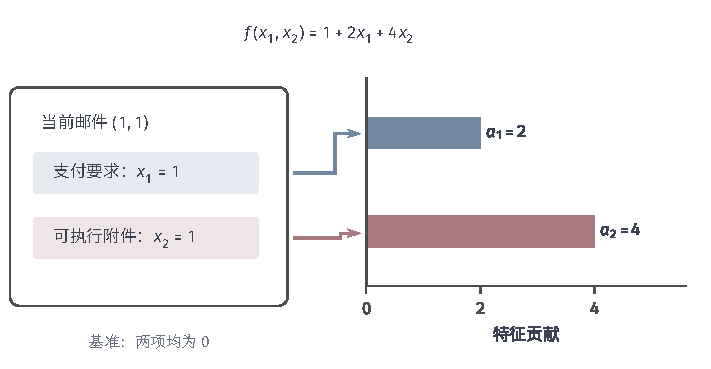
\includegraphics[width=120.407mm]{figures/03-foundations/03-trustworthiness/tikz/trust-feature-attribution/figure.pdf}
  \caption{相对$(0,0)$的教学特征贡献。基准1与当前7相差6，直线路径梯度恒为$(2,4)$，因此IG贡献为2与4。输入标记对应从零起的贡献条，邮件文字只表示规定的二元特征。归因解释分数差，未给出概率或现实因果结论。}
  \label{fig:trust-feature-attribution}
\end{figure*}

另一种分配思路来自合作博弈：把特征看成“玩家”，比较加入不同特征组合时输出的增量，再把每个特征在所有可能加入次序中的边际增量平均，得到它的贡献。设特征集合$N=\{1,\ldots,d\}$，$\mu(S)$表示按规定的缺失填充方式、只保留子集$S$中的当前特征时的平均输出，并假设各联盟平均输出有限。把背景输出$b=\mu(\varnothing)$单独列出，令$v(S)=\mu(S)-b$（于是$v(\varnothing)=0$），第$j$个特征的Shapley贡献为
\begin{equation}
 \phi_j=\sum_{S\subseteq N\setminus\{j\}}
 \frac{|S|!(d-|S|-1)!}{d!}
 \bigl[v(S\cup\{j\})-v(S)\bigr]\, .
 \label{eq:interpretability-shapley}
\end{equation}
SHAP（Shapley additive explanations）就是用这种博弈论分配形成加性贡献\scite{lundberg2017shap}：完整输入的贡献之和等于$f(\bm x)-b$，背景输出$b$作为截距。关键是缺失特征如何填充、用什么分布填充，这决定了$\mu(S)$、基准$b$以及整个解释在回答什么问题（博弈论背景可参考\BookChapterRef{chap:game-theory-and-multi-agent-decision}{卷2《数学准备：概率、因果与决策》第7章“多方策略的响应与演化”}）。

两种填充回答不同问题。边缘填充背景时，$\mu(S)=\mathbb E[f(\bm x_S,\bm X_{-S})]$主要比较模型在人工组合上的响应；$v(S)=\mu(S)-b$只是减去同一个背景常数，不改变各项加入时的增量。若按已知特征条件采样（保留特征间关联），结果会保留关联结构，但也可能把贡献分给一个模型并未直接读取、却能预测其他特征的变量；无论哪种都要按同一背景输出中心化。精确枚举全部联盟是指数规模，用结构性质或采样近似时应报告背景设定与计算误差。

排列式的直观算法是：从背景出发，按某个次序逐个加入当前特征，记录每项加入前后的价值增量，再对所有进入次序平均；特征很多时用采样近似次序。式~\eqref{eq:interpretability-shapley}算的正是这个平均。它与IG的区别要记住：Shapley比较的是离散特征组合的加入增量，IG比较的是连续路径上的梯度积分；两者产物虽然都叫“贡献”，定义并不相同。

\begin{example}[共同信息的贡献分配]
\label{ex:interpretability-redundancy}
示例~\ref{ex:interpretability-redundancy}专门说明信息冗余时的分配。设$v(\varnothing)=0$，$v(\{1\})=v(\{2\})=v(\{1,2\})=1$：任一条信息单独就够用，两者互相替代。一项先进入时增量为1、后进入时增量为0，两种次序各占一半，Shapley贡献各为$1/2$。注意：完整输入中删掉任一项价值仍是1，所以“各分一半”不等于“删掉任一项输出就掉一半”——这是对平均边际增量的分配，不是对移除效果的描述。
\end{example}

\paragraph{支持区域的定位}

图像类解释常先定位“画面中哪些区域支持了目标类别”。梯度加权类激活映射（Grad-CAM）用目标分数对卷积特征图的空间梯度的平均值给各通道加权，再合成一张粗粒度的定位图。设第$k$个通道的特征图为$\bm A^k$、空间位置数为$Z$、目标类别分数为$s_c$，通道权重和定位图为
\begin{equation}
 \begin{aligned}
 \alpha_k^c&=\frac{1}{Z}\sum_{i,j}
 \frac{\partial s_c}{\partial A^k_{i,j}},\\
 L^c_{i,j}&=\max\!\left(0,\sum_k\alpha_k^c A^k_{i,j}\right)\, .
 \end{aligned}
 \label{eq:interpretability-gradcam}
\end{equation}
其中梯度给出每个通道对当前分数的敏感性，特征图给出空间响应，两者合成的是粗粒度位置证据\scite{selvaraju2017gradcam}。

Grad-CAM与IG定位不同：Grad-CAM定位某层表示中支持类别的空间区域，IG把基准分数差分配给输入维度。Grad-CAM受层分辨率、通道梯度平均和只保留正响应（ReLU截断）的限制，会漏掉反对类别的证据和通道内部差异；把低分辨率热力图上采样到原图后，其边缘不能支持像素级因果主张。判断质量时应比较不同类别和对照区域的定位图，而不能仅凭热力图“看起来罩住了物体”就认为解释正确。

\subsection{基于预测计算过程的解释}
\label{sec:interpretability-local-mechanism}

输入响应回答“哪些信息与输出有关”，内部机制解释则固定参数，检验内部的表示、组件和通路如何参与计算。两者的证据强度不同：能从某个激活中解码出信息，只说明该表示含有这些信息；只有替换、屏蔽或恢复该激活后观察到行为变化，才检验了它在计算中的作用。内部干预也可能制造出正常运行中不会出现的异常状态，所以要设置匹配的对照。

一种代表性实验叫激活替换（activation patching）或因果追踪：先保存一次干净运行，再构造一个使目标行为受损的输入运行，然后把干净运行中某个位置的激活复制到受损运行的同一位置，看行为是否恢复。如果输出恢复，就支持“该位置在当前设置中承担了相关计算”。Meng 等用这类实验定位事实关联，并结合参数编辑进一步检验假设\scite{meng2022rome}；但单个激活可能携带多个因素、其他通路也可能冗余保存了同一信息，所以局部恢复不能证明信息唯一存储在该位置。

实验分别记录干净、受损和单位置替换三次运行的分数$s_{\mathrm{clean}}$、$s_{\mathrm{corrupt}}$、$s_{\mathrm{patch}}$。当$s_{\mathrm{clean}}>s_{\mathrm{corrupt}}$时，把恢复差相对原始差归一化为
\begin{equation}
 r_{\mathrm{restore}}
 =\frac{s_{\mathrm{patch}}-s_{\mathrm{corrupt}}}
        {s_{\mathrm{clean}}-s_{\mathrm{corrupt}}}\, ,
 \label{eq:interpretability-restoration}
\end{equation}
教学值4、0、3代入得到$(3-0)/(4-0)=0.75$，意思是这次替换恢复了四分之三的分数差；它不能解释为“该位置存储了75\%的知识”。该比例可以为负或超过1，分母很小时也会剧烈波动。位置恢复图还要在其他输入配对和对照位置上重复测试。

图~\ref{fig:activation-patching}对应这三次运行：第三行在第二行的受损输入上，把干净运行同层同位置的激活复制过来后继续前向，所有运行参数固定。

\begin{figure*}[htbp]
  \centering
  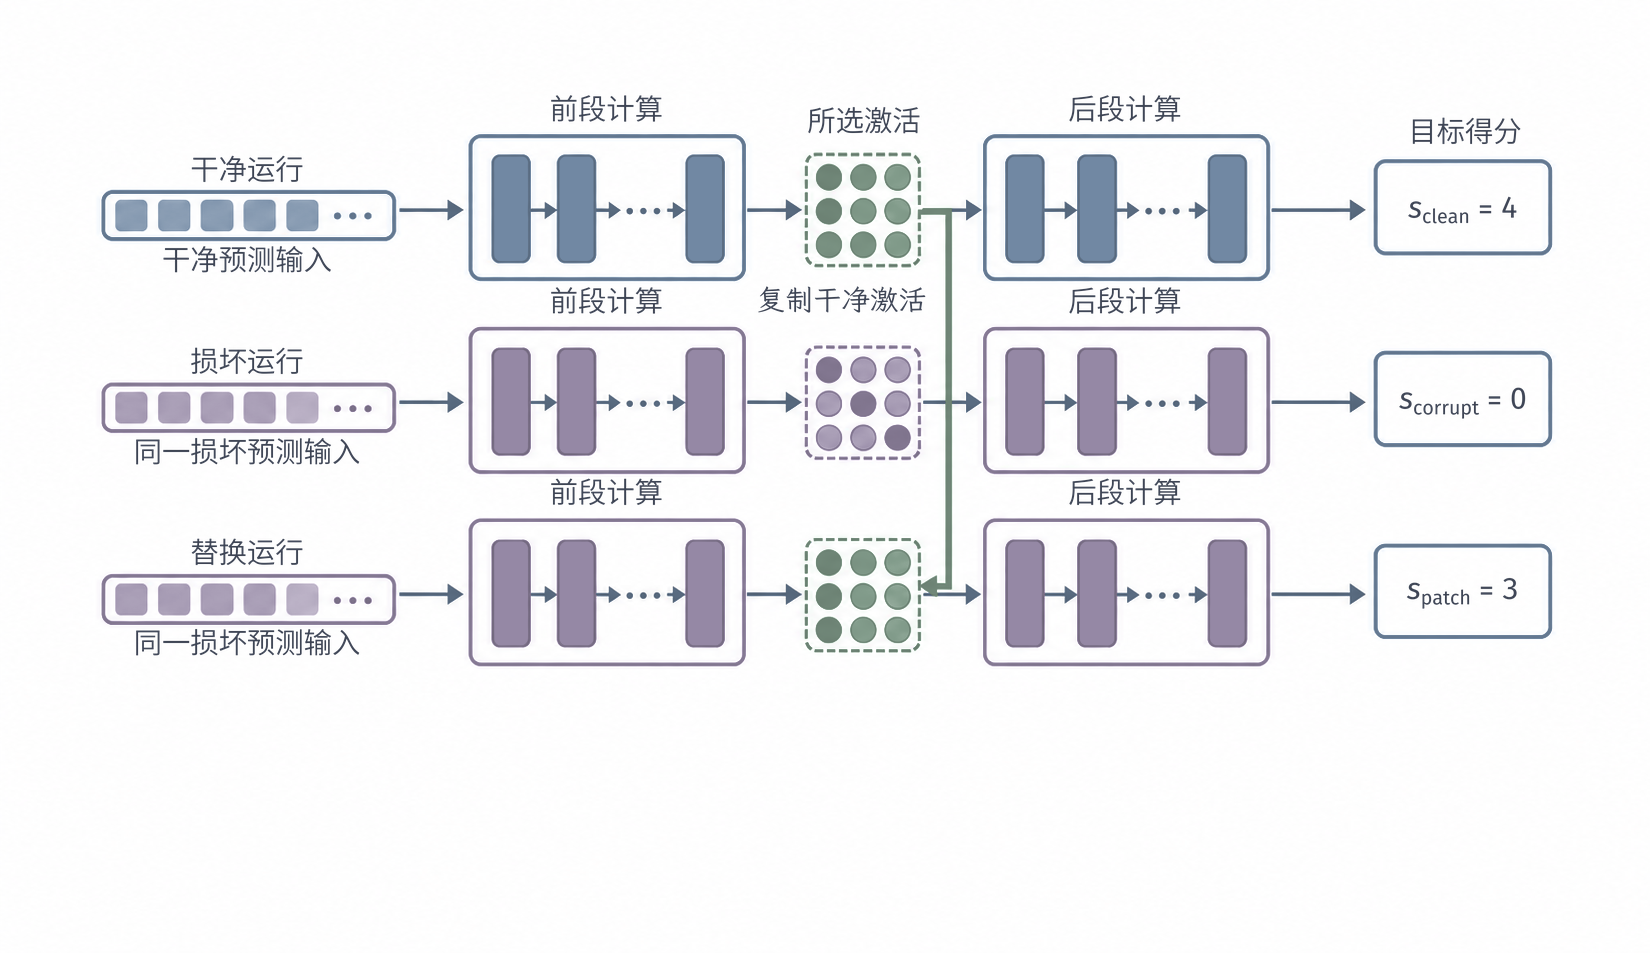
\includegraphics[width=164.600mm]{figures/03-foundations/03-trustworthiness/generated/activation-patching/figure.png}
  \caption{固定参数下的激活恢复试验。第三行保留第二行的受损输入，将干净运行的激活复制到同层同位置后继续前向；教学分数4、0、3给出恢复比例0.75。比例只描述此次分数恢复，不能计量知识或证明唯一位置。绿色复制线与第二行灰色计算线在跨线处不相连。}
  \label{fig:activation-patching}
\end{figure*}

输入归因（IG、遮挡等）分配的是输入维度的作用，机制干预检查的是改变内部计算后行为是否变。两者都可能用到激活或梯度，划分依据是主张的对象：Grad-CAM主要交付空间区域定位，激活替换交付的是“操作某个内部组件的后果”。归因方法提出的机制假设（如“模型靠某区域判断”）还需要干预实验检验，不能直接当成机制结论。

两类干预结论方向不同：移除某组件后行为消失，支持该组件在当前设置中的必要性；把干净激活填回受损运行后行为恢复，支持它在特定背景中的恢复作用。两者都受输入污染方式、替换位置和评分目标限制。多对输入重复、用等强度的随机替换作对照、做组合消融，可以排除一部分替代解释；但单次恢复仍不足以重建完整计算过程。

对工具调用型代理和长生成，解释单位要从单次前向扩展到状态和动作序列：先确定最终行为指标，再定位证据是在哪一步引入的，替换或屏蔽该步状态后重放后续过程，检查任务结果是否改变。序列干预的结论范围以该运行条件为限；最终文本看起来正常也可能掩盖中间某个动作的错误。

\subsection{基于训练样本的解释}
\label{sec:interpretability-local-training}

如果怀疑这次误拦根源是训练集中某个标注错误的样本，解释方向就要转到学习过程：固定当前这封邮件，改变训练样本的特征、标签或权重，重新学习后看预测如何变化。前面的输入解释和内部解释都固定模型参数，这里追溯的是“学习过程如何产生这些参数”。因此“某个训练样本的影响”和“在当前邮件里删词的效果”属于完全不同的实验，不能混为一谈。

最直接的做法是删除可疑样本后重新训练，但对大模型成本太高。\term{影响函数}（influence function）用局部最优解对样本权重的导数来近似这种变化，避免真的重训。为固定归一化尺度，先考虑没有额外缩放正则项的平均目标
\[
 \hat R(\bm{\theta})=\frac1n\sum_{i=1}^n\ell(z_i,\bm{\theta}),
 \qquad
 \bm H=\nabla_{\bm{\theta}}^2\hat R(\hat{\bm{\theta}})\, ,
\]
其中$\hat{\bm{\theta}}$是局部最优解，$\bm H$是该处的海森矩阵，要求$\bm H$可逆、各损失在解的邻域内二阶连续可微。把训练目标改成$\hat R(\bm\theta)+\epsilon\ell(z,\bm\theta)$（相当于给样本$z$加权），沿附近的平稳点分支$\hat{\bm\theta}_\epsilon$对一阶条件求导，可以得到参数随权重的变化率
\[
 \left.\frac{\mathrm d\hat{\bm{\theta}}_\epsilon}
 {\mathrm d\epsilon}\right|_{\epsilon=0}
 =-\bm H^{-1}\nabla_{\bm{\theta}}
       \ell(z,\hat{\bm{\theta}})\, .
\]
为什么这个式子能近似“删掉一个样本”？取$z=z_i$时，按$n-1$归一化的删样本目标与$\hat R-\ell(z,\bm\theta)/n$只差一个不影响极小点位置的常数倍；因此令$\epsilon=-1/n$作一阶外推，删掉样本$z$后参数的变化近似为
\[
 \hat{\bm{\theta}}_{-z}-\hat{\bm{\theta}}
 \approx\frac1n\bm H^{-1}\nabla_{\bm{\theta}}
 \ell(z,\hat{\bm{\theta}})\, .
\]
这个近似成立的条件要列明：解是局部唯一的、损失足够光滑、目标缩放与推导一致；带正则项时尺度要重新推导。样本量少、单个样本影响很强、解不唯一或训练路径本身改变，都会使一阶近似失效。Koh 与 Liang 研究了其在预测追溯上的应用，但实际数据归因仍需部分重训练或受控修改来复核\scite{koh2017influence}。

再对测试样本$z_*$的损失作一阶展开，删掉训练样本$z$对$z_*$损失的影响近似为
\[
 \ell(z_*,\hat{\bm{\theta}}_{-z})
 -\ell(z_*,\hat{\bm{\theta}})
 \approx\frac1n\nabla_{\bm\theta}\ell(z_*,\hat{\bm\theta})^\top
 \bm H^{-1}\nabla_{\bm\theta}\ell(z,\hat{\bm\theta})\, .
\]
内积取负号对应“增加”该样本权重时的局部变化。要强调这个量是由梯度内积定义的，不是输入相似度：内容相似的邮件如果梯度方向不同，影响可以完全不同；内容不相似的错标样本也可能显著移动决策边界。大模型可用海森—向量积迭代求解这个线性系统而不显式求逆，但计算技巧不消除“局部最优”这个前提。

如果训练根本没有收敛到稳定最优点（影响函数前提不成立），可以改用 TracIn 直接追踪训练过程中各次更新的作用。单样本梯度下降中，一次更新使测试损失下降的一阶近似为
\[
 \ell(z_*,\bm\theta^{(t)})-\ell(z_*,\bm\theta^{(t+1)})
 \approx\eta_t
 \nabla\ell(z_*,\bm\theta^{(t)})^\top
 \nabla\ell(z_i,\bm\theta^{(t)})\, .
\]
其中$\eta_t$是学习率，两个梯度都对参数求。Pruthi 等在保存的训练检查点上累积这类内积，估计哪些训练样本有助于降低测试损失、哪些在增加损失\scite{pruthi2020tracin}。它避免了最终海森求逆，但依赖检查点密度、步长、批处理和优化器，也不等同于“从头删掉该样本重训”的真正反事实。

\section{解释的质量}
\label{sec:interpretability-quality}

拿到一条解释（热力图、规则、案例、归因……）之后，不能因为它看起来合理就采信。解释质量要分五个方面独立检查：它与模型真实行为是否相符（保真度）；它在数值和行为范围上覆盖得全不全（完整性与覆盖）；在合理重复下结论稳不稳定（稳定性）；目标读者能不能正确理解（可理解性）；它在实际使用中有没有带来帮助（使用有效性）。这五方面构成不同证据链，应分别取证，不能合成一个笼统的“解释质量分”。

验收前先要固定六件事：模型版本、被解释的输出、声明范围、基准或干预方式、使用者和用途；再预设指标、比较对象、容忍误差、样本与重复范围、不确定性如何报告、失败时如何处理。不同论断需要不同实验——例如删除一条特征曲线既不能统一验证整体规则、也不能验证训练影响。下面按解释对象选择检查，具体阈值由用途决定。

图~\ref{fig:trust-explanation-quality-radar}只展示两套教学方案在保真度、覆盖和稳定性三个维度上实际纳入了几项检查，作用是提示证据缺口；人员理解和使用收益不在图内，需要另外实验。

\begin{figure}[!htb]
  \centering
  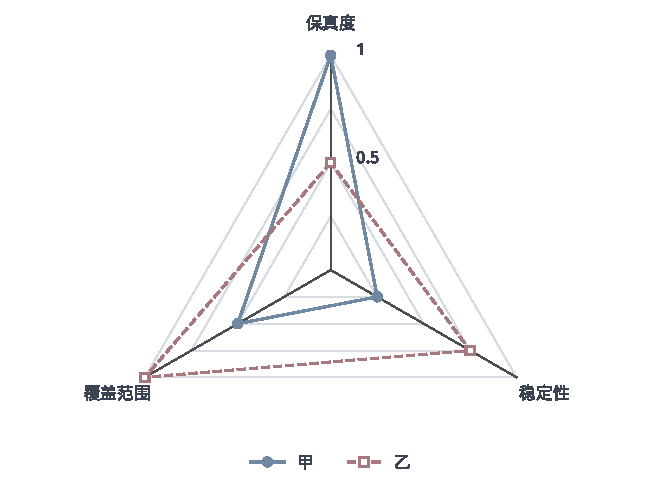
\includegraphics[width=\linewidth]{figures/03-foundations/03-trustworthiness/matplotlib/trust-explanation-quality-radar/figure.pdf}
  \caption{两套构造方案纳入的检查项数。三个维度各预设四项，甲纳入4、2、1项，乙纳入2、4、3项，径向值为项数除以4，线型和标记区分方案。真实检查需预先说明内容与难度；图中面积不合成质量评分，另两项人员与使用评价仍须执行。}
  \label{fig:trust-explanation-quality-radar}
\end{figure}

\subsection{保真度}
\label{sec:interpretability-quality-fidelity}

\term{保真度}（fidelity）度量解释与它所声称描述的模型行为是否一致。要先破除一个直觉：保真度和模型本身的正确率是两回事——一个错误的模型也可以被忠实地解释，解释如实描述了它为什么错。因此保真度要与预测正确率分别报告；它也不同于因果图理论中的 faithfulness 条件，只是同名。

对案例解释，先核查近邻的距离和输出是否真的满足当初声明的检索定义，再确认这些案例是否真的参与了预测（近邻投票权重、原型权重应能重算）；事后检索来的案例若声称“共同因素是判断依据”，必须改变该因素检验响应。仅仅“案例确实相似”只验证了检索环节。

反事实解释要通过完整系统（不是近似代理）复算出目标结果，并报告距离、改动字段数和成立条件。声称某因素“不可缺少”时，应撤销该因素再比较组合；还应主动寻找其他近似方案，检查是否存在选择偏向。方案在现实中是否可执行属于行动补救，预测翻转只回答模型层面的条件。

代理模型在独立查询样本上比较原模型$f$与代理$g$的差异。对非负权重$w_i$，标量分数可用加权平方误差
\[
 \widehat E_{\mathrm{fid}}
 =\frac{\sum_i w_i\,[f(\bm{x}_i)-g(\bm{x}_i)]^2}
        {\sum_i w_i},\qquad \sum_iw_i>0\, .
\]
整体代理的权重应对应声明的参考范围，局部代理（LIME）的权重对应当前邻域。复述类别可用一致率衡量，复述概率还要看分数误差；并应按业务分组检查，避免均值掩盖某个关键分支上的大误差。容差要预先设定，在独立样本上报告区间或重采样波动，超限时应收窄声明范围或拒绝交付，而不是放宽容差。

归因方法要把“定义上的一致性”和“干预下的预测效果”分开验收。IG 检查贡献和是否等于分数差，SHAP 检查背景与缺失规则是否按声明实现；若进一步主张“高贡献因素更关键”，则要做干预实验：按贡献排序逐步删除特征，与随机顺序、低贡献优先顺序对照，也可从基准逐步插入。曲线和面积支持的是相应扰动规则下的效果，分配公理并不保证在所有删除规则下该排序都最优。

扰动实验要匹配改动量和替换方式，并检查改动后输入是否仍然有效：删词可能改变语义、遮挡可能产生异常图像块，这些都会混淆结论。支持证据和反对证据要分别检查（移除被模型依赖的负证据后分数上升，有时正符合归因，不是错误）。整体曲线和概念摘要则在新参考样本上复算，看重要差异是否稳定复现。

Adebayo 等用一种巧妙的 sanity check 检验显著性图：把模型参数随机化、或用打乱的标签重新训练，如果解释图与在原模型上得到的几乎一样，说明图主要反映的是网络结构或边缘先验，而非学到的机制\scite{adebayo2018sanity}。结论要限定在被测方法和设置上，不能据此说所有显著性方法都无效。

参数随机化只排除“解释与机制无关”这一类缺陷。机制解释还应能预测新输入对上的内部屏蔽或恢复效果，并使用随机位置、等强度替换作对照；训练影响类解释则应对高影响、低影响和随机影响样本分别重新加权或部分重训，核对方向和大小。检验改变的对象必须与解释的主张一致。

模型自己生成的文字理由本身也是待验收输出，流畅的叙述可能是事后编造的。如果关键证据改变后模型行为变了、理由却原样不变，就削弱了“理由解释当前依据”的主张。因此要用实验把理由和行为连起来；语言清晰流畅只能验证表达质量。

\subsection{完整性与覆盖范围}
\label{sec:interpretability-quality-coverage}

“完整性”在解释里有两个含义，不要混淆。一是分数差分配意义上的完整：归因各部分是否把相对基准的差正好分完。对有加性要求的归因可计算
\[
 e_{\mathrm{sum}}
 =\left|f(\bm{x})-f(\bm{x}_0)-\sum_j a_j\right|\, ,
\]
其中$a_j$是第$j$项归因。IG用积分求积残差检查这个量，SHAP则要按它定义的$v(\varnothing)$和$v(N)$核对；Grad-CAM没有这种求和承诺，不能要求它满足。零残差只证明约定的数值被分完，仍然没有覆盖全部内部通路、也没有覆盖现实原因。

第二个含义是行为范围的覆盖。规则和代理应按语言、任务类型和重要错误预先分组，报告每组样本量、近似误差和“能被该解释覆盖的比例”；解释器允许弃权时，要同时报告已解释样本的质量和总体覆盖率，避免它只挑简单样本解释。公式能在未测区域算出结果，不构成该区域的解释证据。

机制解释的覆盖更严格：单位置恢复只在当前实验中成立，要把它扩大成“这一类行为都经过该位置”的结论，必须在多个输入、不同表达和组合中复测局部假设，并量化无法被该位置解释的剩余效应。

\subsection{解释的稳定性}
\label{sec:interpretability-quality-stability}

稳定性检验要先固定“哪些条件应当保持不变”，再比较解释结论的波动是否超过预设容限。固定模型、输入、基准和定义后，重复邻域采样、背景采样和概念方向拟合可以测量算法本身的随机性：归因可报均值和标准差，特征排序可报秩相关，前$k$个重要特征可报交并比；比较前应先匹配可交换的编号或方向。

任务规定的等价变换提供另一类稳定性测试。图像区域平移后，应先把归因区域映回原坐标再比较；文本改写（不改变语义）后，应把词元级、词语级或片段级解释转换到同一语义单位，避免把分词变化误判为归因变化。输出类别不变时模型也可能更换了依据，因此这类差异要结合响应分析判断。计算重复、输入迁移和重新训练后的复现应分别报告，它们是三件不同的事。

稳定不等于“无论怎么动都不变”。把模型参数随机化后解释若依然不变，更可能说明解释与模型无关，而不是“稳定的好解释”；一个声称只解释函数本身的方法，对两个实现同一函数的不同系统应给出相容结论。只有预先规定哪些项应保持、哪些项应改变，才能排除“恒定输出图”造成的伪稳定。

\subsection{可理解性}
\label{sec:interpretability-quality-comprehensibility}

可理解性的判据是目标读者是否正确理解了解释，而不是解释本身有多短。规则条数、树深度、非零系数个数和概念熟悉度都只是阅读负担的代理量；一条短而含糊的规则未必比一个明确但稍长的计算更好懂。

人员实验可以让读者根据解释去预测模型对新输入的反应、判断条件变化后的结果，或指出解释的适用范围，记录正确率、用时和误解类型，并匹配任务难度、所需事实和读者背景。例如在教学规则下让读者判断$(0,1)$是否隔离，可以直接检查他是否理解了加性计算和阈值；“我觉得这条解释很清楚”这类主观评分不能替代这种客观检验。

Doshi-Velez 与 Kim 把评价分成三个层次：在真实应用中由应用人员评价、在简化任务上由人员评价、以及不需要人的替代指标\scite{doshivelez2017rigorous}。规则少、归因稀疏这类替代指标便于测量，但是否对应真实理解仍需人员任务提供证据。

实验指令要分清测的是什么能力：让人预测“模型会不会拦截”，检验的是对模型的理解；让人判断“这封邮件应不应该拦截”，还涉及他自己的任务判断能力；实际纠错和错误采纳则是下一节的使用效果。“喜不喜欢这条解释”只反映主观感受。这三类观察不能互相替代。

实验设计上，解释组和对照组应获得相同的必要事实，否则解释组表现好可能只是因为被告知了额外事实：可以保持事实不变、只改变组织方式，或单独设置一个“附加事实”对照。开发者和收件人的背景、任务不同，合适的解释粒度应分别验证。

\subsection{使用有效性}
\label{sec:interpretability-quality-utility}

使用有效性检验解释在实际决策中是否帮人发现模型错误、减少对错误建议的采纳或更好地选择复核，同时计入时间和认知成本。理解模型只是前提，真正的收益要在接近真实的决策任务中评价；补救行动的执行效果在第~\ref{sec:interpretability-recourse-validation}节单独检验。

实验可比较三种配置：无解释、提供所提解释、提供信息量相等但不按解释组织的说明；匹配任务难度，记录最终损失、成功纠错数、错误否决数（把对的也改掉）和用时。题目随机分配或顺序平衡以减少记忆影响。模型错误建议被采纳的比例要单列：整体采纳率上升也可能来自人对模型的过度信任。

一个教学例说明“纠错多不等于结果好”。两组各处理100封匹配邮件，模型都错20次：解释组成功纠正15次但同时新引入8个错误，最终错误为$20-15+8=13$；对照组纠正10次、只新引入1个错误，最终错误为$20-10+1=11$。解释组动作更多但最终错误反而更多。实际比较还需足够样本估计差异的不确定性。

五个维度构成不同证据链，前一项成立不自动推出后一项：解释可以很忠实但人看不懂，看得懂也可能不帮助决策。简化带来的取舍应指出具体维度和输入范围。交付解释时还应明确接收者是谁、要完成什么判断或行动。

\section{行动补救}
\label{sec:interpretability-recourse}

知道了“为什么被拦”之后，使用者真正需要的是一条能恢复业务的可执行路径，这正是反事实解释止步的地方。“不同结果的反事实比较”只找到了“把输入改成什么样模型会改判”，但没有说这个人现实中能不能、以及怎样实现这种改变。\term{行动补救}（algorithmic recourse）寻找在执行者权限和现实后果约束下、真正能达到目标的行动；它要额外考察权限、流程负担、公平性和现实验证（相关因果概念可参考\BookChapterRef{chap:causal-inference}{卷2《数学准备：概率、因果与决策》第3章“因果响应”}）。

补救分三步：先确定可行行动和真实目标（15.5.1），再在约束中比较方案、选择成本合适的（15.5.2），最后核验方案是否真的被执行、结果是否真的达标（15.5.3）。行动的现实后果决定有没有解，成本决定在多个解中选哪个，现实验证决定模型里算出的可行能否真正落实。

\subsection{补救行动的确定}
\label{sec:interpretability-recourse-target}

可行行动首先由执行者的权限决定。发送方可以纠正自己的来源记录、补充证明材料或转换附件格式；收件人可能只能请求复核；运营方则可以修正系统的提取错误或调整流程。一方能做的操作不能直接推荐给另一方。

候选路径有三个来源：纠正记录、改变现实条件、走流程申诉。前两类通常以新输入重新进入模型判断，第三类还改变决策流程本身，应说明由谁处理、依据是什么、时限多长。进入人工复核也不是简单把模型分数调低，而是换一套决策程序。

补救目标必须包含真实任务，而不只是让模型改判。删掉付款要求可能让邮件放行，但同时也删掉了正常的业务请求，这不算成功补救；目标应同时包含“被恰当处理”和“重要内容保留”。如果用户想要的是复核，就应检验是否真的进入并完成了复核流程，而不是强求模型立刻给出有利分类。

每个候选行动都应列出执行者、作用对象、所需资源、时长和预期变化。例如“由发送方把附件转换成既保留必要信息又无可执行内容的格式后重新提交”才构成一个可实施方案；“把附件改成非可执行”这种只在输入表上成立的描述不算。解释提供线索，领域知识和权限决定线索能否执行。

为描述现实后果，设当前状态为$\bm x$、行动$a$造成的新状态为$T(\bm x,a)$，它刻画各字段及其他相关状态如何随行动变化。固定决策规则时新结果是$\hat y(T(\bm{x},a))$；走流程复核则要另行定义结果函数。这里的关键认识是：输入空间里距离小，不代表行动成本低（改一个数字字段 vs 真的去接受一年培训）；在记录里改写某个字段也未必改变它所代表的现实事实。

\subsection{补救行动的选择}
\label{sec:interpretability-recourse-action}

行动集合由不可变属性（如年龄不可改）、权限、允许的变化方向和取值范围限定；后果又受预算、截止时间和业务内容约束。像“合同信息必须保留”这类条件应作为硬约束；可行方案之间在时间、费用上的偏好才进入目标函数。筛选可行方案和对方案排序是两件不同的事，由约束和成本分别承担。

令允许行动集为$A(\bm x)$、行动成本为$c(a;\bm x)$、目标输出集合为$Y_{\mathrm{goal}}$。在固定决策规则下找最低成本方案即
\begin{equation}
 \begin{aligned}
 \min_{a\in A(\bm{x})}\quad &c(a;\bm{x})\\
 \text{满足}\quad &\hat y(T(\bm{x},a))\in Y_{\mathrm{goal}}\, .
 \end{aligned}
 \label{eq:interpretability-recourse}
\end{equation}
四个对象分工清楚：$A$规定哪些行动允许，$T$计算行动的现实后果，输出约束检验后果是否达标，$c$只在达标方案之间比较优劣。只有在目标约束下存在可行行动才谈得上补救；“最优”则依赖所声明的行动范围、后果模型和成本，脱离这些条件不能推广。

成本要对应真实负担：时间、费用、次数可以分列，合成一个标量时要解释权重。一个方案的各项成本都不高于另一个方案、且至少一项更低时，前者支配后者；不同人偏好不同（有人更在意时间、有人更在意费用）时，可以提供若干互不支配的方案供选择。资源约束变化也可能改变最优方案。

Ustun 等把哪些变量可行动、允许往哪个方向变、离散取值和成本写进一个整数规划，在线性分类器下搜索能达到目标的行动，并分析哪些个体根本找不到方案\scite{ustun2019recourse}。这使“翻转输入”落实成一个有明确行动约束的问题。

候选少时可以枚举后果与成本；连续和离散混合的行动可在适用模型下规划或搜索。找到一个可行解只能证明存在这样的解，有限搜索失败不证明无解；声称全局最优需要完备搜索或有效的最优性界，否则应老实声明搜索范围。

行动后果往往相互关联，不能在输入表里把各字段当独立旋钮。例如参加培训提升技能的同时占用时间，可能反而降低当期可投入资源。Karimi 等用结构因果模型计算一个干预沿其后继变量传播的全部影响，再在行动空间里优化成本\scite{karimi2021interventions}。

\begin{example}[约束与成本决定补救方案]
\label{ex:interpretability-causal-recourse}
示例~\ref{ex:interpretability-causal-recourse}把“模型翻转”和“现实可达”的差别讲透。教学规则$s+r\geq3$批准，$s$技能、$r$当期资源，当前$(1,1)$被拒。在输入表里直接把技能记录改成2就能翻转模型，但现实中培训$a\geq0$实际造成$s'=1+a$、$r'=1-a/2$（培训占用资源），总分变成$2+a/2$，需要$a\geq2$才达标；若培训上限为1，仅靠培训永远无法达标。

在培训上限为1的条件下再允许资源支持$0\leq b\leq1$，令$r'=1-a/2+b$，组合成本$c(a,b)=a+3b$。达标要求是$a/2+b\geq1$：只给支持$(0,1)$成本3，培训与支持组合$(1,1/2)$成本2.5，两者都达标。

在这些条件下，可行解满足$b\geq1-a/2$，代入成本得$c=a+3b\geq3-a/2\geq2.5$（用了$a\leq1$），组合$(1,1/2)$恰好达到这个下界，因而是最优方案。如果预算只有2，那么所有允许组合的最低成本都高于预算，数学上无解——这个“无解”是从后果方程和成本下界推出来的，不是搜索没搜到。
\end{example}

图~\ref{fig:trust-actionable-recourse}对比“只改技能记录”的虚假路径和真实行动路径：培训$a=1$先到$(2,1/2)$，再加支持$b=1/2$才到批准边界。行动可行性同时取决于权限、后果和预算，模型翻转只是其中一项条件。

\begin{figure}[htbp]
  \centering
  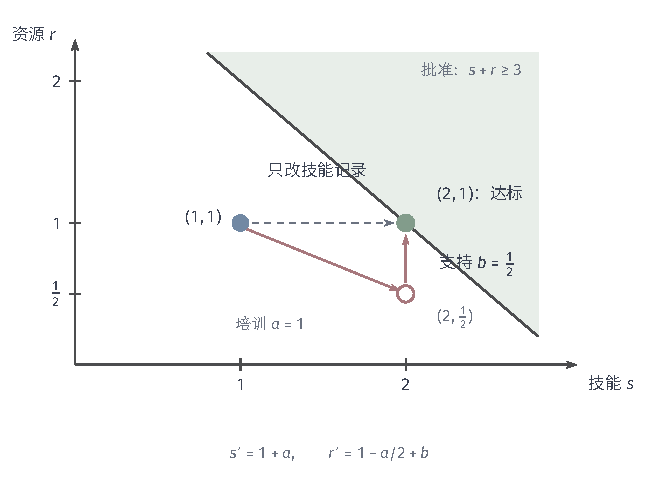
\includegraphics[width=\linewidth]{figures/03-foundations/03-trustworthiness/tikz/trust-actionable-recourse/figure.pdf}
  \caption{示例~\ref{ex:interpretability-causal-recourse}的约束补救组合。虚线表示只改技能记录；培训$a=1$实际先到$(2,1/2)$，支持$b=1/2$再到批准边界。仅培训且上限为1无法达标，组合成本2.5；预算为2时，成本下界证明允许集合中无可行方案。}
  \label{fig:trust-actionable-recourse}
\end{figure}

后果或未来模型不确定时，可以要求候选方案在一组有依据的情形中都达标（稳健补救），或在明确的概率模型中达到预设成功率。容限取自任务风险；收紧要求通常会增加成本，也可能导致无解。出现无解时应定位到底是预算、权限、后果还是规则造成的限制，再考虑放宽或走复核，而不是随便推荐一个方案。

还要区分“有一个后果模型能算出结果”和“现有证据足以识别后果”。多套结构因果模型可能符合同样的观察、甚至同样的边缘干预数据，却对某个个体的后果给出不同预测。正确做法是先声明证据和领域知识允许的模型类，再报告方案、成本和成功概率对模型选择的敏感性，必要时加模型类上的稳健约束。识别依据缺失不能简单当成一个参数误差忽略。

\subsection{补救效果的验证}
\label{sec:interpretability-recourse-validation}

补救验收分两层，证据不能互替。计算层核对方案是否满足约束和目标（在模型里可行），执行层比较行动实施后的真实后果（现实中有效）。第~\ref{sec:interpretability-quality-utility}节检验解释怎样影响人的判断，这里检验行动实施后的结果；用户满意度不能同时替代这两种证据。

\paragraph{方案与约束的复核}

计算层：对方案重新核查权限、不可变属性、取值范围、时限和预算，再用$T$产生新状态，通过真实的特征处理和决策流程重新计算（代理或连续近似给出的候选必须回到真实系统验证）。成本最优性可以用穷举、精确求解小规模问题或有效的求解界来复核；无法证明最优时要明确报告限制。

在教学例中代入组合$(1,1/2)$得到新状态$(s',r')=(2,1)$、总分3、成本2.5，且满足行动上限，这证明它在模型内可行且达标；成本下界则另外证明它最优。若预算只有2，这个达标候选依然不可执行。

\paragraph{行动后果与实际收益的检验}

执行层：实际记录应包含行动是否完成、费用、真实状态变化和最终目标达成情况。把新状态与$T$的预测对照，才能发现后果模型是否高估。技能和资源的观察相关性通常不足以预测个人培训效果，应结合干预证据、对照研究和执行记录检验假设，并限定结论支持的范围。

一个后果模型失效的例子：如果实际中每单位培训消耗的资源是0.8而非假设的0.5，执行组合$(1,1/2)$后真实状态是$(2,0.7)$，总分只有2.7，仍未达标。计算本身符合所设模型，失效完全来自后果假设错误。这时应重新估计$T$、重新求方案，而不能引用原来的“最优性证明”声称现实有效。

评价补救方法时应分别报告三个比例：建议中可行的比例、实际被完成的比例、完成后真正达标的比例，以及费用和不利后果，且每项都要写清分母。只统计“执行成功的人”会遗漏两类人——根本没有可行方案的、和有方案但无法执行的。按群体报告无解、完成、成功、等待时间和成本分布，可以发现群体差异和申诉负担；但这些汇总本身不能说明差异是否沿不可接受的属性路径产生，因果路径要另建机制核验（口径见第~\ref{chap:trust-fairness}章）。声称建议带来收益时，还要与无建议或既有方式对照，并处理是否采纳建议的自选择差异。

验收最终要回到业务目标：邮件放行了但合同内容损坏、某指标分数降了但实际风险还在，都不算完成补救。复核和申诉要观察实质处理、错误是否纠正和时间负担，决策变化与真实收益要分别报告。

\paragraph{效果保持与失效处理}

补救需要时间，因此方案应标明所依据的模型版本、后果假设和有效条件。周期较长时模型更新或环境变化可能使方案失效，应在有依据时重算或跟踪实施结果；有限情形的验证不能保证所有未来条件。

形成一个修订循环：无法完成操作时修订行动集，实际后果与预测不符时修订$T$，规则或流程变化时重新检查目标；然后重新生成候选、重新求解带约束的优化问题，并用新的执行记录验证。对最终仍无可行方案的个体，应给出明确的限制说明和可用的复核途径，而不是给一个注定失败的建议。

\section{本章小结}
\label{sec:interpretability-summary}

回到章首的三个问题。整体规则描述一整组邮件的判断规律，单次证据定位当前这封邮件为什么被拦，结构、输入和语义解释分别交代计算如何组合、具体因素起什么作用、这些因素对应什么含义。即使结合使用，每一项主张的范围仍要分别写明。

单次解释可以沿三个方向取证：输入响应（案例、反事实、局部代理、归因，模型固定）、内部计算（干预激活与组件，改变运行）、学习经历（影响函数、TracIn，改变学习）。要记住贡献数字可以复算不等于机制已经确定，内部通路不等于现实因果；把局部结果汇总成整体结论前，还必须检验子群异质性和覆盖范围。

解释的五类质量分别对应模型行为、声明范围、合理重复、目标读者和实际使用任务，各需独立证据。行动补救还需要权限、现实后果模型和因果识别依据，并核查不同群体的机会和成本负担。最后两点伦理边界：清晰的解释也可能如实揭示一个错误的或不公平的依赖，这正是前面几章要处理的问题；而展示训练经验和私人特征本身会引入信息披露风险，引出下一章的隐私保护。

\paragraph{扩展阅读}

Doshi-Velez与Kim的框架可用于区分人员实验和替代指标；LIME与积分梯度则适合比较邻域代理和基准贡献所支持的不同主张。阅读时沿评价对象与证据条件分析，而非仅比较可视化外观\scite{doshivelez2017rigorous,ribeiro2016lime,sundararajan2017ig}。

反事实解释与因果补救可对照阅读。Wachter等搜索邻近目标输入，Karimi等加入行动及连带后果；两条路线分别验证预测条件与行动方案，其差别来自待优化对象\scite{wachter2018counterfactual,karimi2021interventions}。
